\chapter{Background}
\label{sec:background}
%
In this chapter bla bla
\todo{Describe Chapter}

% ===========================================
% ===========================================
% Autonomic computing
% ===========================================
% ===========================================
\section{Autonomic computing}
Autonomic computing is an architecture for computing systems to enable the ability to manage themselves in accordance to high level objectives configured by administrators \cite{Kephart2003VisionComputing}. 
These computing systems dynamically adapt to demands and conditions of the workload \cite{Kephart2003VisionComputing}.
An intelligent control-loop is responsible to collect all important details of the computing system and make decision according to the collected details. To automate the tasks, the intelligent control-loop is organized into four categories:

\begin{itemize}
\item \textbf{Self-configuring}
- Components in the environment have to adapt dynamically to system changes using policies. For example, deploying or removing new components.

\item \textbf{Self-healing}
- If system errors have being detected, the control-loop has to perform policy-based actions without disrupting the 
environment.

\item \textbf{Self-optimizing}
- The control-loop has to monitor the resources and should adapt to changes dynamically.

\item \textbf{Self-protecting}
- Detection and protection against threats.

\end{itemize}

 An autonomic computing environment consists of an autonomic manager, managed-resources and a knowledge-base.
 % As shown in figure ...
 
\subsection{Managed resources}
Managed resources are software or hardware components in the computing environment. For example, a managed resource 
can be a database, service, application, server or different entity. Each managed resource implements an interface to enable 
the autonomic manager to communicate with the managed resource. 

These interface are called touchpoints.

\subsection{Autonomic manager}
The autonomic manager implements an intelligent control-loop to collect system metrics from the managed resources and acts according to the collected details. It can only make adjustments within it`s own scope and uses policies to make decisions of what actions have to be
executed to accommodate the objectives.
To be self-managing, the autonomic manager has to implement the following four automated functions.

\begin{itemize}
\item \textbf{Monitor}
- The monitor function is responsible to collect the needed metrics from all managed resources and applies aggregation and filter
operations to the collected data. After that the function reports the metrics.

\item \textbf{Analyze}
- To determine if changes have to be made to the computing system, the collected data has to be analyzed.

\item \textbf{Plan}
- If changes have to be made, an appropriate change plan has to be generated. A change plan consists of actions that are needed to achieve the configured goals and objectives. The change plan needs to be forwarded to the execute function.

\item \textbf{Execute}
- The execute function applies all necessary changes to the computing system.

\end{itemize}

Multiple autonomic manager can exist in an autonomic computing environment to perform only certain parts. For example, 
there can be one autonomic manager which is responsible to monitor and analyze the system and another autonomic manager 
to plan and execute. To create a complete and closed control-loop, multiple autonomic manager can be composed together.


% ===========================================
% ===========================================
% Docker
% ===========================================
% ===========================================
\section{Docker}
% Short docker intro
Docker is an open-source platform that enables containerization of applications. Containerization is a technology to package, ship and run applications and their environment in individual containers.
% Make clear
Docker is not a container technology itself, it hides the complexity of working with container technologies directly and instead provides an abstraction and the tools to work with containers \cite{Nickoloff2019Docker, Bullington2020Docker, Potdar2020Docker}.


\subsection{Docker architecture}

% Architecture figure
\begin{figure}[h]%
\centering
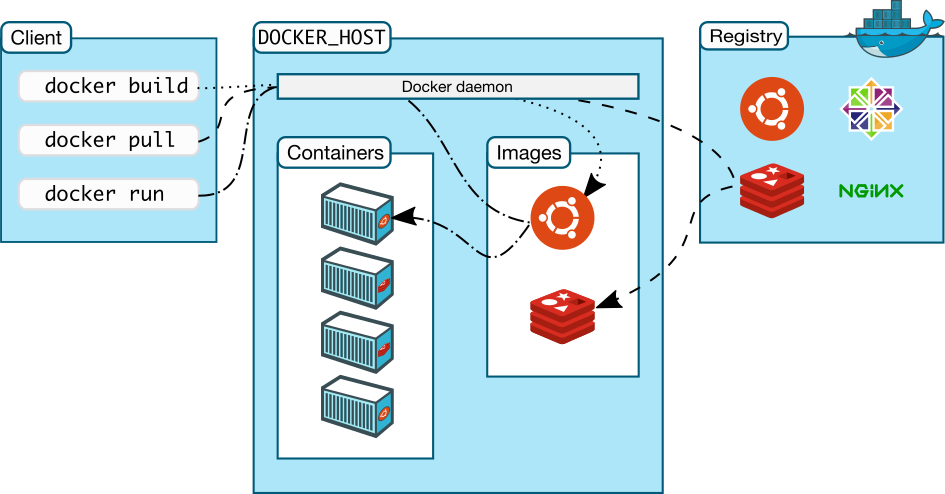
\includegraphics[scale=0.5]{images/03_background/docker_architecture}%
\caption{Docker architecture - Source: Authors own model, based on \cite{Docker2020Docs}.}%
\label{fig:spark_docker_architecture}%
\end{figure}

% Explain figure
\Fig{fig:spark_docker_architecture} illustrates the client server architecture of Docker which consists of of a Docker client, the Docker deamon and a registry.


\paragraph{Docker client:} The Docker client is an interface for the user to send commands to the Docker deamon \cite{Docker2020Docs}.


\paragraph{Docker deamon:} The Docker deamon manages all containers running on the host system and handles the containers resources, networks and volumes \cite{Bullington2020Docker}.


\paragraph{Docker Registry:} A Docker registry stores images. Images can be pushed to a public or private registry and pulled from it to build a container \cite{Docker2020Docs}.


\subsection{Docker image}
% What is an image
An Image is a snapshot of the environment that is needed to run an application in a Docker container. The environment consists of all files, libraries and configurations that are needed for the application to run properly \cite{Docker2020Docs, Nickoloff2019Docker}.
% How to create an image
Images can be created from existing containers or from executing a build script called Dockerfile. A Dockerfile is a text file consisting of instructions for building an image. The Docker image builder executes the instructions of a Dockerfile from top to bottom \cite{Nickoloff2019Docker}.

% Dockerfile example
\begin{lstlisting}[frame=single, label=lst:docker_dockerfile, caption=Example of a Dockerfile, captionpos=b]
FROM ubuntu:latest

RUN apt-get update && apt-get install -y git

ENTRYPOINT ["git"]
\end{lstlisting}

% Example Dockerfile example
\Lst{lst:docker_dockerfile} provides an example of a Dockerfile with three instructions.
\begin{enumerate}
\item \texttt{FROM ubuntu:latest} - This image is build on top of the latest Ubuntu image. Dockerfiles have to start with a \texttt{FROM} instruction \cite{Nickoloff2019Docker}.
\item \texttt{RUN apt-get update \&\& apt-get install -y git} - Update the package manager and install Git.
\item \texttt{ENTRYPOINT ["git"]} - Set the git command as the entrypoint of this image.
\end{enumerate}

% How to build an image
\todo{Vielleicht noch erklären wie Images mit Docker build erstellt werden.}


\subsection{Docker Container}
% What are containers
A container is an execution environment running on the host-system kernel.

% Container image
\begin{figure}[h]%
\centering
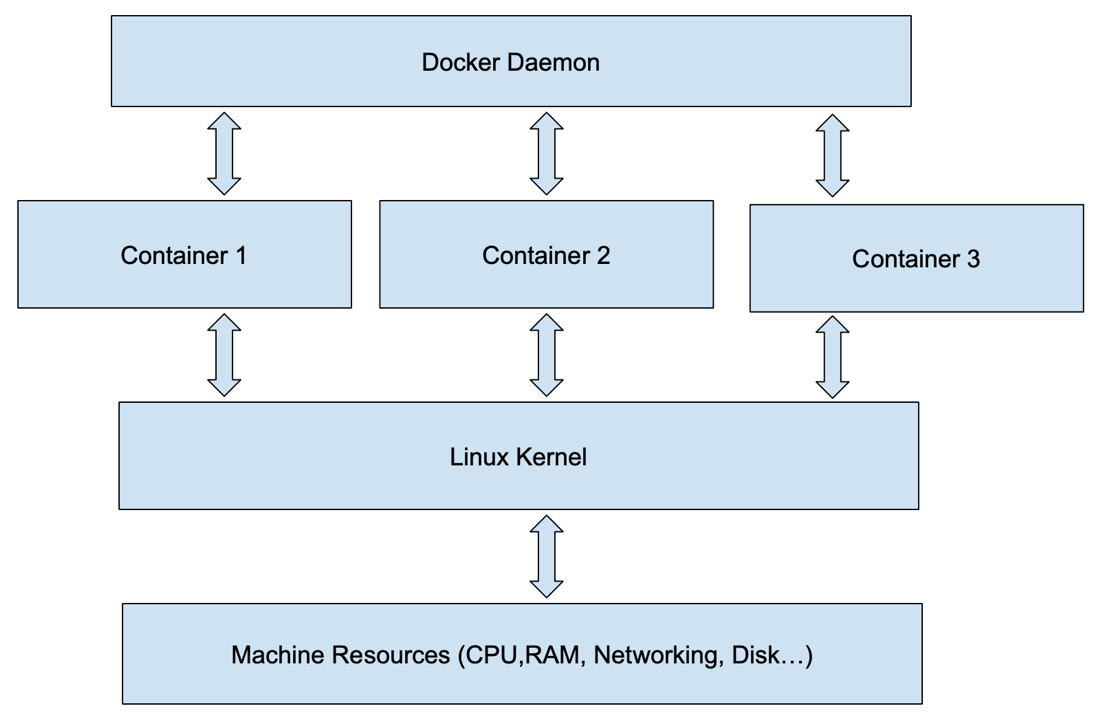
\includegraphics[scale=0.8]{images/03_background/docker_basic_container_structure}%
\caption{Docker basic container structure - Source: Authors own model, based on \cite{Bullington2020Docker}.}%
\label{fig:docker_container_struct}%
\end{figure}

% Container advantages
The advantage of a container is its lightweight nature. As illustrated in \Fig{fig:docker_container_struct}, containers take advantage of OS-level virtualization instead of hardware-virtualization without the need of a hypervisor \cite{Docker2020Docs, Nickoloff2019Docker}. Containers share the resources of the host-system instead of using reserved resources \cite{Bullington2020Docker}. Multiple containers can run on the host-system kernel and are by default isolated from each other \cite{Docker2020Docs}.
% Docker container
In Docker, a container is a runnable unit of an image and is used for distributing and testing applications. A container can be configured to expose certain resources to the host system, e.g. network ports \cite{Bullington2020Docker}.


\subsection{Docker Compose}
% What is compose
Docker Compose is a tool to run multi-container applications on a single host. A multi-container application consists of a stack of services, where each service is deployed as a container \cite{Bullington2020Docker, Docker2020Docs}.
% How does compose works
Services can be configured in a YAML\footnote{YAML Ain't Markup Language - https://yaml.org/} file called \textit{docker-compose.yml}. This file defines the requirements of each service and determines how a service communicates to other services \cite{Kane2018DockerUp}.


% ===========================================
% ===========================================
% Apache Spark
% ===========================================
% ===========================================
\section{Apache Spark}
Apache Spark is an open-source computing framework for parallel data processing on a large computer cluster. Spark manages the available resources and distributes computation tasks across a cluster to perform big-data processing operations at large scale \cite{Chambers2018Spark}. Before Spark was developed, Hadoop MapReduce \cite{Dean2010MapReduce} was the framework of choice for parallel operations on a computer cluster \cite{Zaharia2010Spark}. Spark accomplished to outperform Hadoop by 10x for iterative Machine Learning \cite{Zaharia2010Spark}. It is implemented in Scala\footnote{Scala programming language. https://www.scala-lang.org/}, a JVM-based language and provides a programming interface for Scala, Java\footnote{Java programming language. https://www.oracle.com/java/}, Python\footnote{Python programming language. https://www.python.org/} and R\footnote{R programming language. https://www.r-project.org/}. In addition, Spark includes an interactive SQL shell and libraries to implement Machine Learning and streaming applications \cite{Chambers2018Spark}.
It was developed in 2009 as the Spark research project at UC Berkeley and became an Apache Software Foundation project in 2013 \cite{Chambers2018Spark}. 


\subsection{Spark programming model}
\label{sec:spark_programming_model}
% Explain RDDs
Spark provides resilient distributed datasets (RDDs) as the main abstraction for parallel operations \cite{Zaharia2010Spark}. Core types of Spark`s higher-level structured API are built on top of RDDs \cite{Chambers2018Spark} and will automatically be optimized by Spark`s Catalyst optimizer to run operations quick and efficient \cite{Hien2018Spark}.
\todo{Master-Slave Architektur + Bild}


\paragraph{Resilient distributed datasets:}
% What are RDDs
Resilient distributed datasets are fault-tolerant, parallel data structures to enable data sharing across cluster applications \cite{Zaharia2012RDDs}. They allow to express different cluster programming models like MapReduce, SQL and batched stream processing \cite{Zaharia2012RDDs}. RDDs have been implemented in Spark and serve as the underlying data structure for higher level APIs (Spark structured API) \cite{Zaharia2012RDDs}.
% How can RDDs be used in applications    !! HIER MAL BEISPIEL WIE IN RDD ERZEUGT WIRD
RDD`s are a immutable, partitioned collection of records and can only be initiated through transformations (e.g. map, filter) on data or other RDD`s.
% What are the advantages of RDDs    !!! HIER NOCHMAL BEISPIEL WIE DAS AUSSEHEN KANN
An advantage of RDDs is, that they can be recovered through lineage. Lost partitions of an RDD can be recomputed from other RDDs in parallel on different nodes \cite{Zaharia2012RDDs}. 
% Better use structured API
RDDs are lower level APIs and should only be used in applications if custom data partitioning is needed \cite{Chambers2018Spark}. It is recommended to use Sparks structured API objects instead. Optimizations for RDDs have to be implemented manually while Spark automatically optimize the execution for structured API operations \cite{Chambers2018Spark}.


\paragraph{Spark structured API:}
% What is the structured API
Spark provides high level structured APIs for manipulating all kinds of data. The three distributed core types are Datasets, DataFrames and SQL Tables and Views \cite{Chambers2018Spark}.
% About DataFrames, Datasets and SQL
Datasets and DataFrames are immutable, lazy evaluated collections that provide execution plans for operations \cite{Chambers2018Spark}. SQL Tables and Views work the same way as DataFrames, except that SQL is used as the interface instead of using the DataFrame programming interface \cite{Chambers2018Spark}.
% Differences between Datasets ad Dataframes
Datasets use JVM types and are therefore only available for JVM based languages. DataFrames are Datasets of type Row, which is the Spark internal optimized format for computations. This has advantages over JVM types which comes with garbage collection and object instantiation \cite{Chambers2018Spark}.


\paragraph{Spark Catalyst:}
% What is the Catalyst optimizer
Spark also provides a query optimizer engine called Spark Catalyst. \Fig{fig:spark_catalyst_process} illustrates how the Spark Catalyst optimizer automatically optimizes Spark applications to run quickly and efficient.
% Short How
Before executing the user`s code, the Catalyst optimizer translates the data-processing logic into a logical plan and optimizes the plan using heuristics \cite{Hien2018Spark}. After that, the Catalyst optimizer converts the logical plan into a physical plan to create code that can be executed \cite{Hien2018Spark}.


% What are logical plans
Logical plans get created from a DataFrame or a SQL query. A logical plan represents the data-processing logic as a tree of operators and expressions where the Catalyst optimizer can apply sets of rule-based and cost-based optimizations \cite{Hien2018Spark}.
For example, the Catalyst can position a filter transformation in front of a join operation \cite{Hien2018Spark}.

% What are physical plans
From the logical plan, the Catalyst optimizer creates one ore more physical plans which consist of RDD operations \cite{Chambers2018Spark}. The cheapest physical will be generated into Java bytecode for execution across the cluster \cite{Hien2018Spark}.

% Spark Catalyst figure
\begin{figure}[h]%
\centering
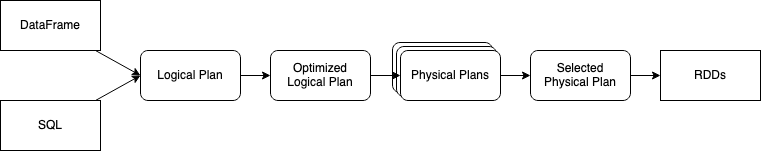
\includegraphics[scale=0.5]{images/03_background/spark_catalyst}%
\caption{Optimization process of the Spark Catalyst - Source: Authors own model, based on \cite{Hien2018Spark}.}%
\label{fig:spark_catalyst_process}%
\end{figure}
\todo{Bild nochmal machen mit abstand	+ QUELLE anpassen}


\subsection{Spark application architecture}

\begin{figure}[h]%
\centering
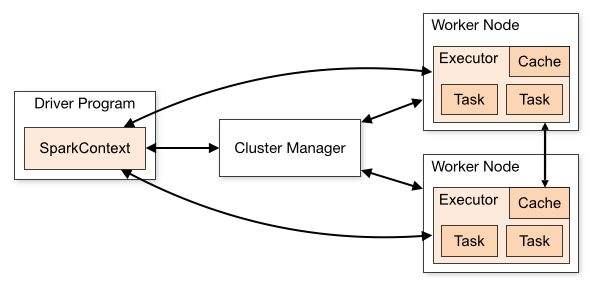
\includegraphics[scale=0.5]{images/03_background/cluster_overview}%
\caption{Overview of a Spark cluster architecture - Source: Authors own model, based on \cite{Apache2020Spark}.}%
\label{fig:spark_cluster_overview}%
\end{figure}

\todo{Lieber Doch Master/Slave ???. Was ist mit dem CLuster-Manager}
% Explain image
\Fig{fig:spark_cluster_overview} illustrates the main architecture of a Spark cluster. The architecture follows the master-worker model where the Spark driver is the master and the Spark executors are the worker \cite{Hien2018Spark}.
\todo{Nicht ganz richtig, Master und Worker sind machines und driver und executor sind prozesse}

\paragraph{Spark driver:}
The Spark driver is a JVM process on a physical machine and responsible to maintain the execution of a Spark application \cite{Chambers2018Spark}. It coordinates the application tasks onto each available executor \cite{Hien2018Spark}. To get launch executors and get physical resources, the Spark driver interacts with the cluster manager \cite{Chambers2018Spark, Hien2018Spark}.


\paragraph{Spark Executor:}
A Spark executor performs the tasks given by the Spark driver \cite{Chambers2018Spark}. It runs as a JVM process and runs until the Spark application finishes \cite{Hien2018Spark}. After the executor finishes, it reports back to the Spark driver \cite{Chambers2018Spark}. Each task will be performed on a separate CPU core to enable parallel processing  \cite{Hien2018Spark}.


\paragraph{Cluster manager:}
The cluster manager is an external service that orchestrates the work between the machines in the cluster \cite{Hien2018Spark, Apache2020Spark}. The cluster manager knows about the resources of each worker and decides on which machine the Spark driver process and the executor processes run \cite{Hien2018Spark, Chambers2018Spark}.
% Different cluster types
Spark supports different services that can run as the cluster manager: Standalone, Apache Mesos\footnote{Apache Mesos. https://mesos.apache.org/}, Hadoop YARN\cite{Murthy2013Yarn} and Kubernetes\footnote{Kubernetes. https://kubernetes.io/} \cite{Apache2020Spark}.
% What is standalone
\todo{Explain standalone}
% Explain different cluster deploy modes
The cluster manager provides three different deploy modes for acquiring resources in the cluster.
\begin{itemize}
\item Cluster mode
\item Client mode
\item Local mode
\end{itemize}

% Cluster mode
To run an application in cluster mode, the user has to submit a precompiled JAR, python script or R script to the cluster manager \cite{Chambers2018Spark}. After that, the cluster manager starts the driver process and executor processes exclusively for the Spark application on machines inside the cluster \cite{Chambers2018Spark, Hien2018Spark}.
\begin{figure}[h]%
\centering
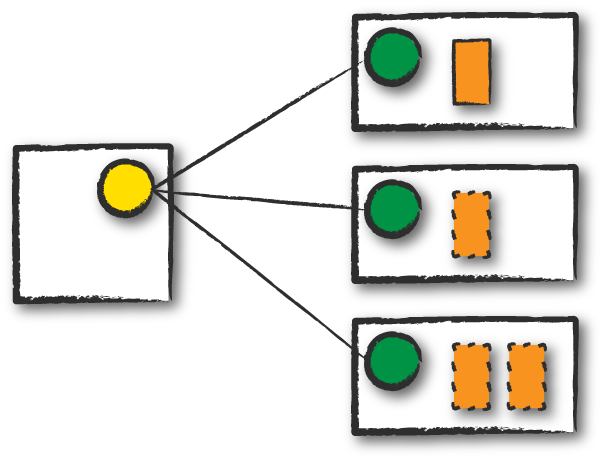
\includegraphics[scale=0.5]{images/03_background/cluster_mode}%
\caption{Spark`s cluster mode - Source: Authors own model, based on \cite{Chambers2018Spark}.}%
\label{fig:spark_cluster_mode}%
\end{figure}

% Client mode
The difference between the client mode and the cluster mode is that, the driver process runs on the client machine outside of the Spark cluster \cite{Chambers2018Spark}.
\begin{figure}[h]%
\centering
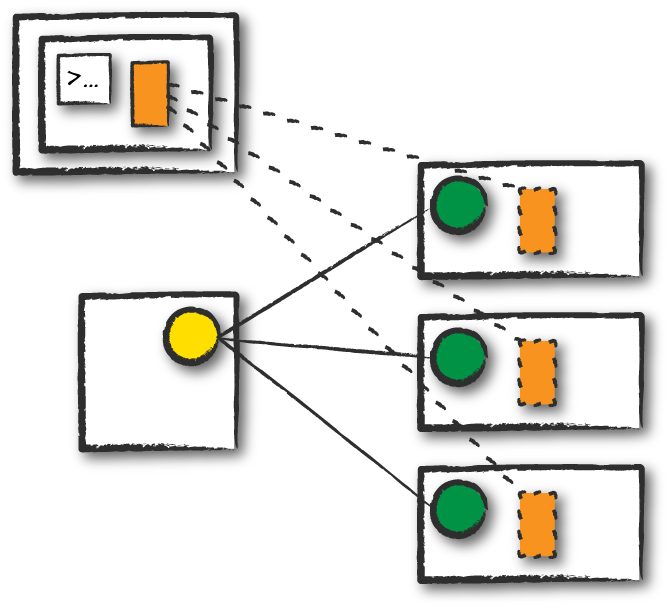
\includegraphics[scale=0.5]{images/03_background/client_mode}%
\caption{Spark`s client mode - Source: Authors own model, based on \cite{Chambers2018Spark}.}%
\label{fig:spark_client_mode}%
\end{figure}

% Local mode
The local mode starts a Spark application on a single computer \cite{Chambers2018Spark}. It is not recommended to use the local mode in production, instead it should be used for testing Spark applications or learning the Spark framework \cite{Chambers2018Spark}.


\subsection{Spark application implementation}
% Short intro
The concept of a Spark application consists of calling transformations and actions. A transformation creates a DataFrame or a Dataset, the logical data structures of a Spark application. The computation of a Spark application gets processed when an action gets called in the application. The transformations of a Spark application build up a directed acyclic graph (DAG) of instructions. By calling an action, the DAG will break down into stages and tasks to create a single job for execution \cite{Chambers2018Spark}.
% Show example application
\begin{lstlisting}[frame=single, label=lst:spark_python_example, caption=Example of a Python3 Spark application, captionpos=b]
# Initialize a SparkSession
sparkSession = SparkSession\
    .builder\
    .getOrCreate()

# Create a dataframe with a transformation
dataframe = sparkSession.range(1, 1000)
# Apply another transformation
dataframe = dataframe.filter(dataframe.id % 2 == 0)
# Call an action
count = dataframe.count()
\end{lstlisting}
% Explain a spark application on top of an example
\Lst{lst:spark_python_example} demonstrates an example implementation of a Spark application. At first a SparkSession gets initialized. Each Spark application must include a SparkSession to initialize the application driver and executors  \cite{Chambers2018Spark}. In Addition, the SparkSession provides an API for data-processing logic and configuration of the Spark application \cite{Hien2018Spark}. After that, a DataFrame gets created with the range transformation to include each number from 1 to 1000 in the DataFrame. Next, a filter transformation is applied on the DataFrame to sort out any odd number. At the end, the number of rows gets saved in a variable with the count action.
\todo{Create listing macro}



% How to submit
\todo{Tabelle von Luu18 vll als Anhang(Table 2-1 Subdirectories Inside the spark-2.1.1-bin-hadoop2.7 Directory)}
The Spark framework provides a spark-submit executable to launch a Spark application inside a cluster.
% Show example submit
\begin{lstlisting}[frame=single, label=lst:spark_submit_example, caption=Execution of a Spark Python application using the spark-submit executable, captionpos=b]
$SPARK_HOME/bin/spark-submit \
    --master spark://spark-master:7077 \
    application.py
\end{lstlisting}
% Explain
\Lst{lst:spark_submit_example} provides an example how the spark-submit executable can be used to launch a Spark Python application.


\subsection{Spark standalone cluster deployment}
% Why only standalone
\todo{Why only standalone}
% What is a standalone cluster
The standalone mode is a basic cluster-manager build specifically for Spark. It is developed to only run Spark but supports workloads at large scale \cite{Chambers2018Spark}.

% How can we create a cluster
Spark provides build-in scripts to start a master node and worker nodes in standalone mode. ABC demonstrates how a master node and worker node gets launched using the build-in scripts.
% NE ALTER !, schon erwähnen start-master und start-worker


% ===========================================
% ===========================================
% NVIDIA RAPIDS
% ===========================================
% ===========================================
\section{RAPIDS accelerator for Apache Spark}
% Explain
The RAPIDS accelerator for Apache Spark is a plugin suite to enable GPU acceleration for computing operations on Apache Spark 3.x \cite{SparkRapids2020Docs}. 
% What it does
To accelerate computing operations, it uses the RAPIDS\footnote{Open GPU Data Science - https://rapids.ai/} libraries and extends the Spark programming model (see \SubSec{sec:spark_programming_model}) \cite{SparkRapids2020Docs, Mcdonald2020SparkRapids}.

\subsection{Extension of the Spark programming model}
% How does it extends DataFrame and SQL
The plugin suite extends the Spark programming model with a new DataFrame based on Apache Arrow\cite{ApacheArrow2020Docs} data structures and the Catalyst optimizer to generate GPU-aware query plans \cite{Mcdonald2020SparkRapids}.


% What is Apache Arrow
Apache arrow is a data platform to build high performance applications that work with large dataset`s and to improve analytic algorithms. A component of Apache Arrow is the Arrow Columnar Format, an in-memory data structure specification for efficient analytic operations on GPUs and CPUs \cite{ApacheArrow2020Docs}.


% How do DataFrames and SQL use RAPIDS
Spark`s DataFrame and SQL use the RAPIDS APIs to run tranformations and actions on a GPU.
% How does the Catalyst create GPU aware plans
The Spark Catalyst optimizer identifies operator in a query plan that are supported by the RAPIDS APIs. To execute the query plan, these operators can be scheduled on a GPU within the Spark cluster \cite{Mcdonald2020SparkRapids}. If operators are not supported by the RAPIDS APIs, a physical plan for CPUs will be generated by the Catalyst optimizer to execute RDD operations \cite{Mcdonald2020SparkRapids}. \Fig{fig:rapids_query_plan} illustrates, how a query plan gets optimized with the RAPIDS accelerator for Spark enabled.

% RAPIDS query plan image
\begin{figure}[h]%
\centering
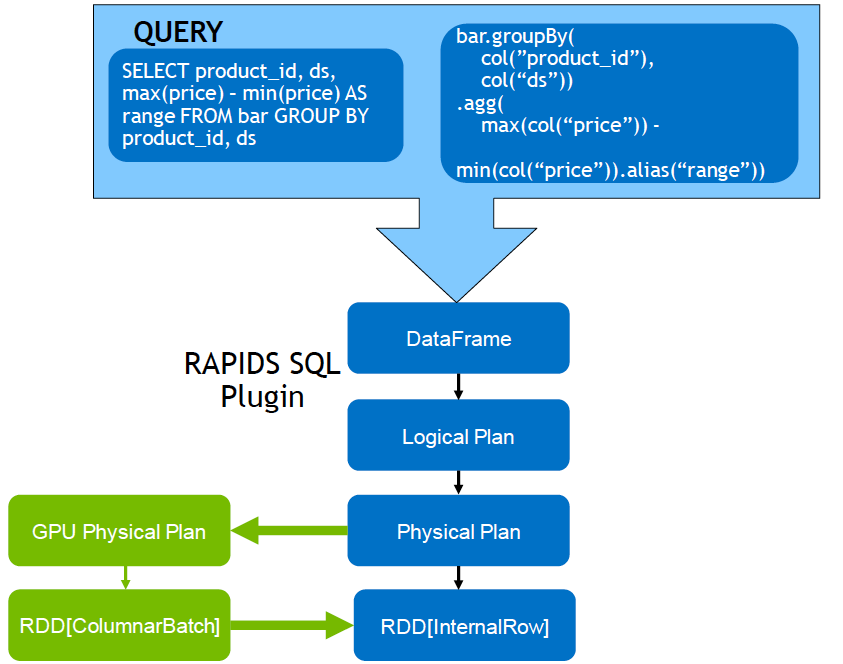
\includegraphics[scale=0.25]{images/03_background/rapids_query_plan}%
\caption{Catalyst optimization with RAPIDS accelerator for Apache Spark - Source: Authors own model, based on \cite{Mcdonald2020SparkRapids}.}%
\label{fig:rapids_query_plan}%
\end{figure}


% ====
% Prometheus
% ====
\section{Prometheus}
% What is Prometheus
Prometheus is an open-source monitoring and alerting system \cite{Prom2020Docs}.
% Time-series format + PromQL
To collect and store data, Prometheus supports a multi-dimensional key-value pair based data model which can be analyzed in real-time using the PromQL query language \cite{Pandey2020Monitoring}.
% Pull-based approach
It follows the pull-based approach to scrape metrics from hosts and services \cite{Bastos2019Prom}.

% Pull-based image
\begin{figure}[h]%
\centering
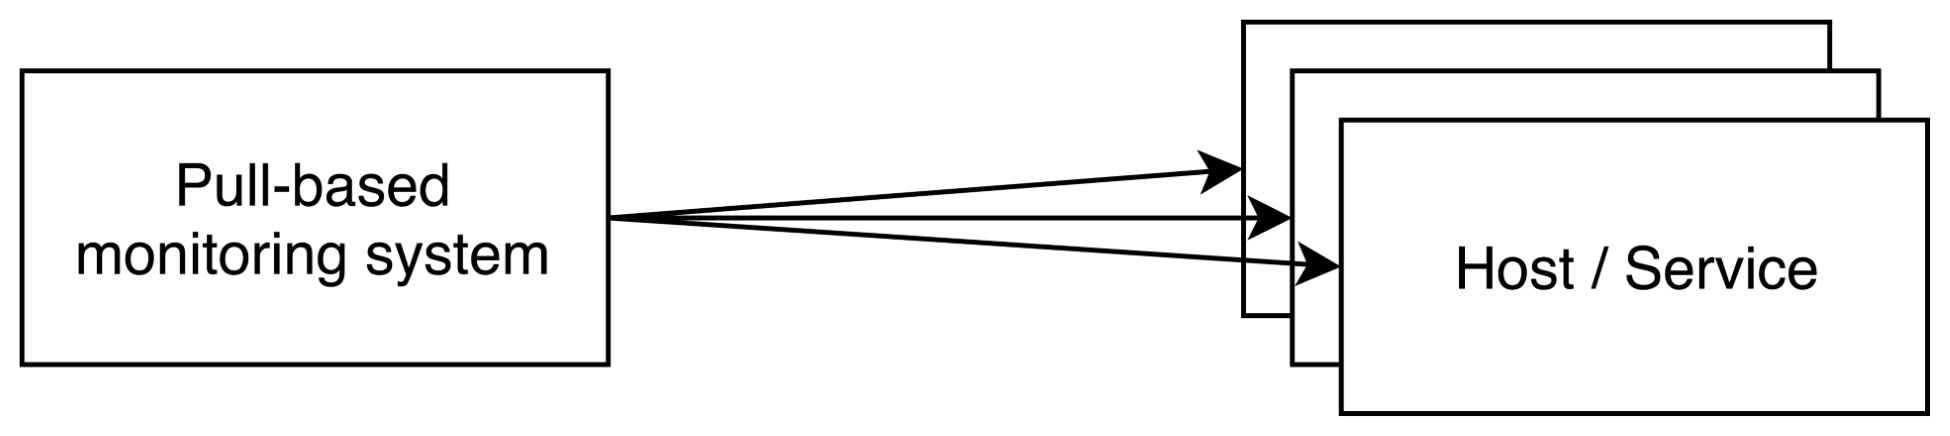
\includegraphics[scale=0.25]{images/03_background/prom_pull-based}%
\caption{Pull-based approach to scrape metrics - Source: \cite{Bastos2019Prom}.}%
\label{fig:prom_pull-based}%
\end{figure}

% Describe figure
As \Fig{fig:prom_pull-based} demonstrates, a pull-based monitoring system scrapes metrics from services which makes them available for the monitoring system. In this case, the monitoring system needs a list of all hosts and services to monitor \cite{Bastos2019Prom}.


% What is monitoring and why is it important
A monitoring system keeps track of the health status of components in a computing cluster. Because of the complexity of modern computing clusters, the effort is to high to observe components manually \cite{Bastos2019Prom}.


% What are metrics
A metric is an observed property of software or hardware, e.g. the usage of a CPU core. To measure metrics, data-point`s will be recorded at a fixed time interval. A data-point is a pair of a value and a timestamp. The combination of multiple data-point`s is called a time-series \cite{Turnbull2016Monitoring}.


\subsection{Prometheus architecture}

\todo{Bilder für components}

% Architecture image
\begin{figure}[h]%
\centering
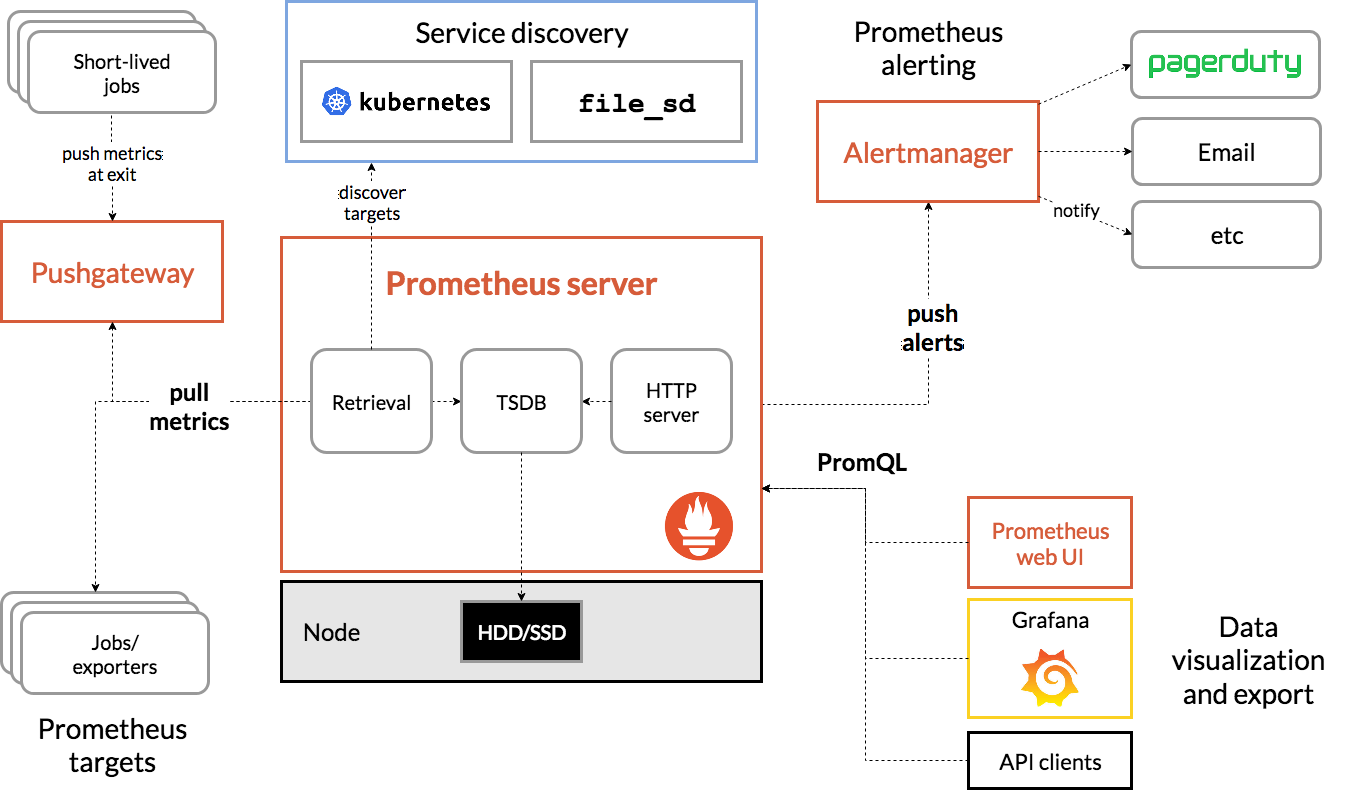
\includegraphics[scale=0.25]{images/03_background/prom_architecture}%
\caption{Prometheus high-level architecture - Source: Authors own model, based on \cite{Prom2020Docs, Bastos2019Prom}.}%
\label{fig:prom_architecture}%
\end{figure}

% High level architecture
\Fig{fig:prom_architecture} illustrates the high-level architecture of Prometheus.
% Description of components
The Prometheus ecosystem provides multiple components. Components can be optional, depending on the monitoring needs of the environment \cite{Bastos2019Prom}. The main components of a Prometheus system are Prometheus server, Alertmanager, service discovery, exporters, Pushgateway and visualization tools \cite{Prom2020Docs}.


\paragraph{Prometheus server:} 
The Prometheus server is the main component of a Prometheus system. It is responsible to collect metrics as time-series data from targets and stores the collected data in the built-in TSDB \cite{Bastos2019Prom}. Prometheus uses the concept of scraping to collect metrics from a target. A target host has to expose an endpoint to make metrics available in the Prometheus data format \cite{Pandey2020Monitoring}. Additionally, the Prometheus server triggers alerts to the Alertmanager if a configured condition becomes true \cite{Prom2020Docs}.


\paragraph{Alertmanager:}
If an alerting rule becomes true, the Prometheus server generates an alert and pushes it to the Alertmanager. The Alertmanager generates notifications from the received alerts. A notification can take multiple forms like emails or chat messages. Webhooks can be implemented to trigger custom notifications \cite{Bastos2019Prom}.


\paragraph{Service discovery:}
As mentioned before, Prometheus follows a pull-based approach to fetch metrics from a target. To know about all targets, Prometheus needs a list of the corresponding hosts. The service discovery manages the complexity of maintaining a list of hosts manually in an changing infrastructure \cite{Bastos2019Prom}.


\paragraph{Exporters:}
If an application does not support an endpoint for Prometheus, an exporter can be used to fetch metrics and make them available to the Prometheus server. An exporter is a monitoring agent running on a target host that fetches metric from the host and exports them to the Prometheus server \cite{Pandey2020Monitoring}.


\paragraph{Pushgateway:}
If a target is not designed to be scraped, metrics can be pushed against the Pushgateway\cite{Prom2020Docs}. The Pushgateway converts the data into the Prometheus data format and passes them to the Prometheus server \cite{Pandey2020Monitoring}.


\paragraph{Visualization:}
Prometheus supports various tools for virtualization of the scraped data. Grafana\footnote{Grafana: The open observability platform - https://grafana.com/} is one of the widely used tools for this occasion.


%\subsection{Creating alerts}
% Beschreiben wie man das mach in der yml datei


\subsection{Monitoring Docker container}
% How can Prometheus be used with Docker (cAdvisor)
% Auch auf andere Technologien eingehen -> Measuring DockerPerformance What a Mess!!!
\todo{Wahrscheinlich erst nach der implementation}


% ===========================================
% ===========================================
% Gitlab CI/CD
% ===========================================
% ===========================================
\section{Gitlab}


% ===========================================
% ===========================================
% K-MEANS
% ===========================================
% ===========================================
\section{K-MEANS}


% ===========================================
% ===========================================
% Bayes
% ===========================================
% ===========================================
\section{Naive Bayes Classifier}


% ===========================================
% ===========================================
% Scaling heat
% ===========================================
% ===========================================
\section{Scaling heat}


% ===========================================
% ===========================================
% KHP
% ===========================================
% ===========================================
\section{KHP}